
\documentclass{tufte-handout}

\makeatletter
\renewcommand{\maketitlepage}{%
\begingroup%
\setlength{\parindent}{0pt}

{\fontsize{24}{24}\selectfont\textit{\@author}\par}

\vspace{1.75in}{\fontsize{36}{54}\selectfont\@title\par}

\vspace{0.5in}{\fontsize{14}{14}\selectfont\textsf{\smallcaps{\@date}}\par}

\vfill{\fontsize{14}{14}\selectfont\textit{\@publisher}\par}

\thispagestyle{empty}
\endgroup
\newpage
}
\makeatother

% Book metadata
\title{An Introduction to Machine Learning}
\date{\today}
\author{Alexandre St-Aubin}
\publisher{McGill University -- Directed Reading Program}

\usepackage{amsmath}
\usepackage{amsthm} %needed for the proofs 
\usepackage{amssymb}
\usepackage{xcolor} %for heading colors
\usepackage{titling}
\usepackage{thmtools}
\usepackage[linesnumbered,ruled,vlined]{algorithm2e} %For pseudocode

%For plots
\usepackage{pgfplots}
\pgfplotsset{compat = newest}

\newtheoremstyle{mytheoremstyle}
    {6pt} % space above
    {6pt} % space below
    {\normalfont} % body font
    {} % indent amount
    {\bfseries} % theorem head font
    {.} % punctuation after theorem head
    {1em} % space after theorem head
    {\thmname{#1}\thmnumber{ #2}\thmnote{ (#3)}} % theorem head spec

\newtheoremstyle{corlstyle}
    {6pt} % space above
    {6pt} % space below
    {\normalfont} % body font
    {} % indent amount
    {\textit{}} % theorem head font
    {.} % punctuation after theorem head
    {1em} % space after theorem head
    {\thmname{#1}\thmnumber{ #2}\thmnote{ (#3)}} % theorem head spec

% Define the theorem environment
\declaretheorem[style=mytheoremstyle,name=Theorem,numberwithin=section]{theorem}

% Define the corollary environment linked to the theorem
\declaretheorem[style=corlstyle,name=Corollary,numberlike=theorem,parent=theorem]{corollary}

\declaretheorem[style=corlstyle,name=Remark,numberlike=theorem]{remark}

\declaretheorem[style=corlstyle,name=Example,numberlike=theorem]{example}

% Define the lemma environment linked to the theorem
\declaretheorem[style=mytheoremstyle,name=Lemma,numberlike=theorem]{lemma}

% Define the proposition environment linked to the theorem
\declaretheorem[style=mytheoremstyle,name=Proposition,numberlike=theorem]{proposition}

% Define the definition environment linked to the theorem
\declaretheorem[style=mytheoremstyle,name=Definition,numberlike=theorem]{definition}

\newcommand\sol{%
  \\ 
  \\
  \textit{Solution:}\\%
}
\newcommand{\indep}{\perp \!\!\! \perp}

\DeclareMathOperator{\var}{Var}
\DeclareMathOperator{\cov}{Cov}

%\geometry{showframe} % display margins for debugging page layout

\usepackage{graphicx} % allow embedded images
  \setkeys{Gin}{width=\linewidth,totalheight=\textheight,keepaspectratio}
  \graphicspath{{graphics/}} % set of paths to search for images

\usepackage{booktabs} % book-quality tables
\usepackage{units}    % non-stacked fractions and better unit spacing
\usepackage{multicol} % multiple column layout facilities
\usepackage{lipsum}   % filler text
\usepackage{fancyvrb} % extended verbatim environments
  \fvset{fontsize=\normalsize}% default font size for fancy-verbatim environments
%\begin{marginfigure}
%  \includegraphics{nonConvex}
%  \label{ConvexExamples2015}
%  \caption{A nonconvex function does not lie below all of its secants.}
%\end{marginfigure}


\usepackage{hyperref}% for better handling of links 
% Prints argument within hanging parentheses (i.e., parentheses that take
% up no horizontal space).  Useful in tabular environments.
\newcommand{\hangp}[1]{\makebox[0pt][r]{(}#1\makebox[0pt][l]{)}}

%%
% Prints an asterisk that takes up no horizontal space.
% Useful in tabular environments.
\newcommand{\hangstar}{\makebox[0pt][l]{*}}

%%
% Prints a trailing space in a smart way.
\usepackage{xspace}

% Generates the index
%\usepackage{makeidx}
%\makeindex

% Standardize command font styles and environments
\newcommand{\doccmd}[1]{\texttt{\textbackslash#1}}% command name -- adds backslash automatically
\newcommand{\docopt}[1]{\ensuremath{\langle}\textrm{\textit{#1}}\ensuremath{\rangle}}% optional command argument
\newcommand{\docarg}[1]{\textrm{\textit{#1}}}% (required) command argument
\newcommand{\docenv}[1]{\textsf{#1}}% environment name
\newcommand{\docpkg}[1]{\texttt{#1}}% package name
\newcommand{\doccls}[1]{\texttt{#1}}% document class name
\newcommand{\docclsopt}[1]{\texttt{#1}}% document class option name
\newenvironment{docspec}{\begin{quote}\noindent}{\end{quote}}% command specification environment


\setcounter{secnumdepth}{4} %to set the section numbering

\begin{document}

\maketitlepage% this prints the handout title, author, and date

% r.5 contents
\tableofcontents
\newpage

\section{Introduction}
There are several types of Machine Learning algorithms. The main categories are divided into \textit{Supervised learning, Semi-supervised learning, Unsupervised learning and Reinforcement learning.} Here, we will focus on \textit{Supervised learning.}
\begin{definition}[Supervised Learning]
  In supervised learning, the machine learns through examples. The machine learning algorithm is tasked with developing the strategy for achieving the specified outputs given some input.  To do so, a known dataset is supplied  that contains a set of inputs and associated outputs. The algorithm finds patterns in the data, learns from observations, and makes predictions. At the end of the learning process, the algorithm can be tested on data that is unknown to it, but that the operator knows the answers to, in order to test its accuracy. Then, the algorithm is adjusted if needed, and the process continues in an iterated manner.
\end{definition}
talk about types of ML problems (classification, regression)
\section{Neural Networks}
Neural networks, a subset of machine learning, form the core of supervised learning and are inspired by the human brain\cite{web:IBM:NN}.They are made of input, hidden, and output layers, and consist of interconnected \textit{neurons} with associated \textit{weights and thresholds}. Activated nodes transmit data to the next layer if their output surpasses the threshold. The overall network is a combination of function composition and matrix multiplication:

  $$g(x) = f^L (W^Lf^{L-1}(W^{L-1} \hdots f^1(W^1x)\hdots)), $$
  where $L$ is the number of layers (\ref{sub:Layers}), $W$ is the weight matrix (\ref{sub:Weights}), and $f$ is the activation function (\ref{sub:ActivationFunction}).

\subsection{Neurons}%
  \label{sub:Neurons}

\begin{definition}[Neurons]
  Neurons are the building blocks of neural networks. They receive an input, multiply it by a weight, and output it using an activation function. A simple mathematical model for a neuron's output activation is\cite{book:AIModernApp}
\begin{marginfigure}
  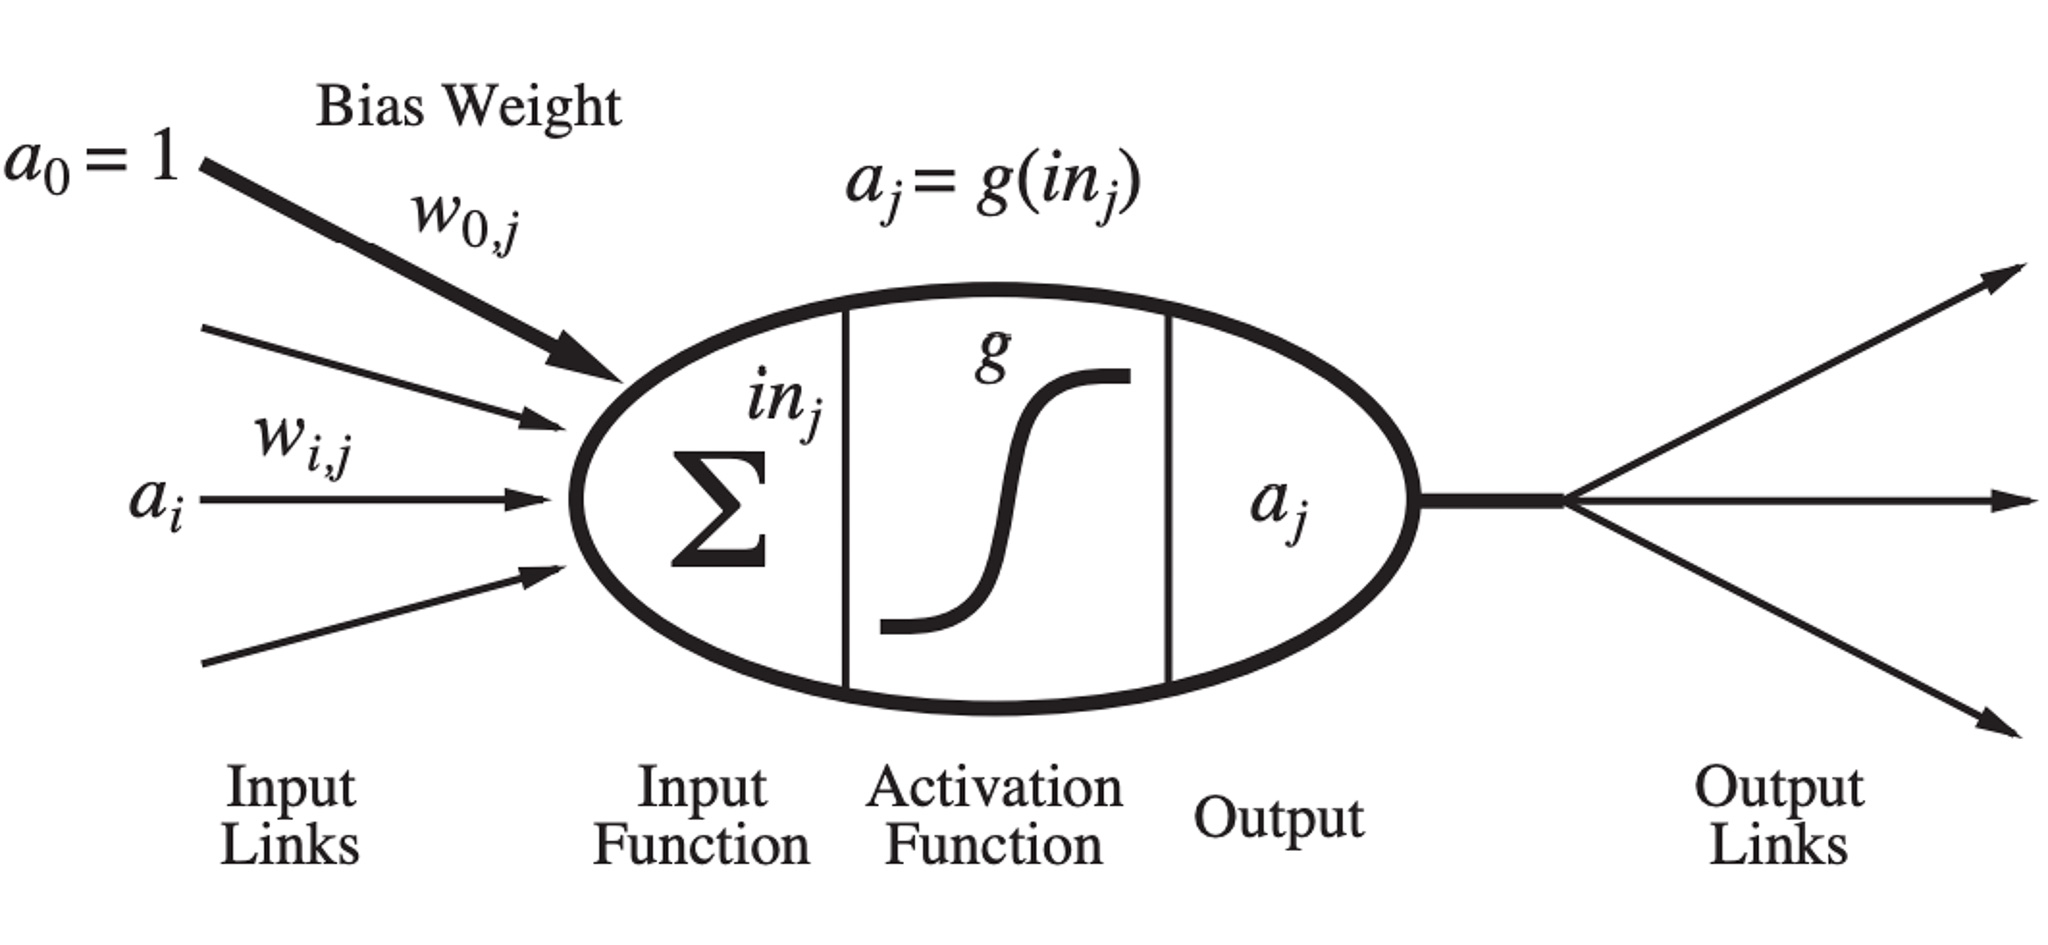
\includegraphics{Neuron}
  \label{Neuron}
  \caption{A neuron and its inputs and outputs.}
\end{marginfigure}
  $$a_j = f \left( \sum^{n}_{i=0}w_{i,j} a_i  \right)$$
  where $f$ is the activation function (\ref{sub:ActivationFunction}), $a_i$ is the output activation of neuron $i$ and $w_{i,j}$ is the weight on the link from neuron $i$ to $a_j$. We will explore activation functions in more depth shortly.  
\end{definition}

  
\begin{definition}[Artificial Neural Networks]
 
\end{definition}
\subsection{Weights}%
  \label{sub:Weights}
  
\subsection{Layers}
\label{sub:Layers}
The layers are divided in 3 groups: the \textit{input, hidden,} and \textit{output} layers. See figure \ref{NeuralNetwork} for an image of the layers. Layers are a general term given to a grouping of neurons that act together in the neural network.
\begin{marginfigure}
  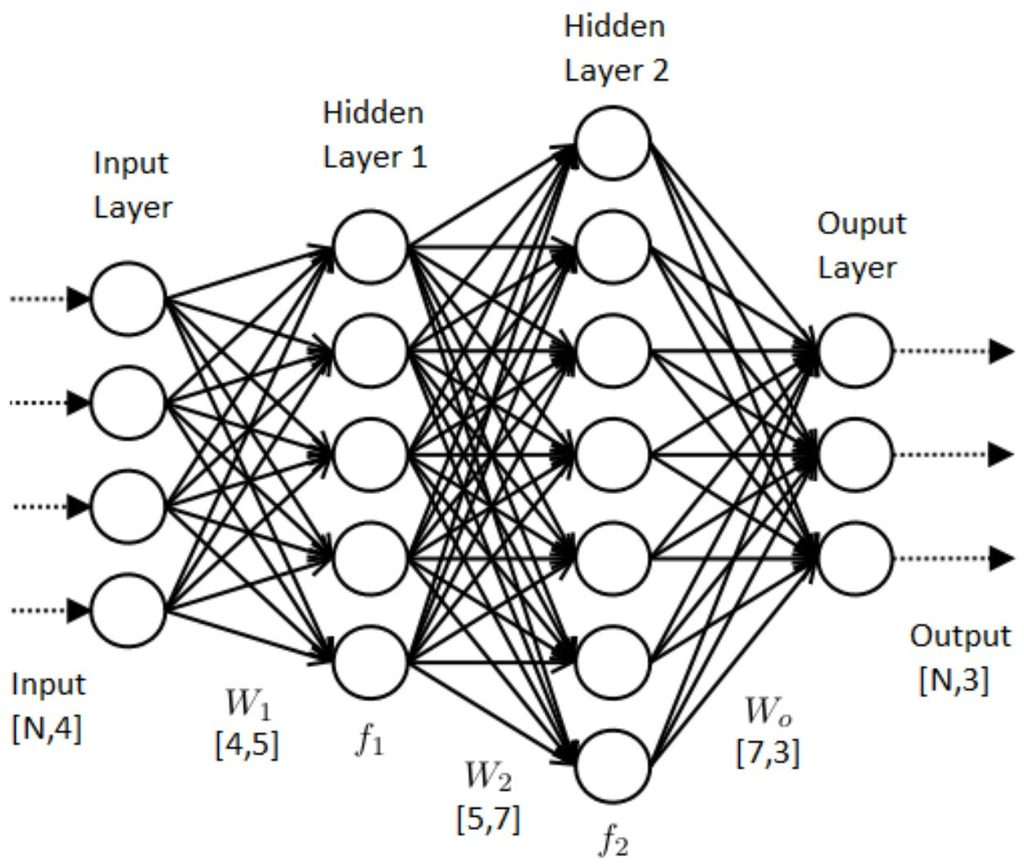
\includegraphics{NeuralNetwork}
  \label{NeuralNetwork}
  \caption{A graph representation of a Neural Network.}
\end{marginfigure}
\begin{definition}[Layers] $  $
  \begin{enumerate}
    \item[\it Input Layer.] The first layer in a neural network, it receives the initial data for the network from the outside world. The "Entry point" of the neural network.
    \item[\it Hidden layers.] The hidden layer(s) are where the magic happens in neural networks. Each layer is trying to learn different aspects about the data by minimizing the \textbf{cost function}. The most intuitive way to understand these layers is in the context of 'image recognition' such as a face. The first layer may learn edge detection, the second may detect eyes, third a nose, etc.\cite{layers}.
    \item[\it Output Layer.] The final layer in the neural network is the output layer. This layer is responsible for holding the final result or output of the problem. Input, such as raw images, is fed into the input layer, and the output layer produces the corresponding result.
\end{enumerate}

\end{definition}

\subsection{Activation Function}%
  \label{sub:ActivationFunction}
An activation function in neural networks is a smooth function applied to the output of each neuron in a layer. It introduces non-linearity to the network, allowing it to learn complex patterns and relationships in the data.

The activation function determines whether a neuron should be activated or not based on the weighted sum of its inputs. In other words, it defines the output of a neuron given a set of inputs. Without activation functions, neural networks would be limited to linear transformations, and they wouldn't be able to capture the non-linearities present in many real-world datasets. 

\vspace{5mm}
\noindent \textbf{Desired Characteristics of Activation Functions} \cite{jagtap2022important}

\noindent There is no universal rule for choosing the best activation function, but there are some characteristics to look for, namely
\begin{enumerate}
  \item[\it Nonlinearity] One of the most essential characteristics
of an activation function is nonlinearity. In comparison
to linear activation functions, the non-linearity of the
activation function significantly improves the learning
capability of neural networks. 
\item[\it Computationally Cheap] The activation function must
be easy to evaluate in terms of computation. This has
the potential to greatly improve network efficiency.
\item[\it Finite Range/Boundedness] Gradient-based training approaches are more stable when the range of the activation function is finite, because pattern presentations
significantly affect only limited weights. 
\item[\it Differentiability] The most desirable quality for using
gradient-based optimization approaches is continuously
differentiable activation functions. This ensures that the
back-propagation algorithm works properly. 
\end{enumerate}
\begin{remark} 
  The vanishing and exploding gradient problems: The variation
of the inputs and outputs of some activation functions,
such as the logistic function (Sigmoid), is extremely
large. To put it another way, they reduce and transform
a bigger input space into a smaller output space that
falls between [0,1]. As a result, the back-propagation
algorithm has almost no gradients to propagate backward
in the network, and any residual gradients that do exist
continue to dilute as the program goes down through the
top layers. Due to this, the initial hidden-layers are left
with no information about the gradients. For hyperbolic
tangent and sigmoid activation functions, it has been
observed that the saturation region for large input (both
positive and negative) is a major reason behind the
vanishing of gradient. One of the important remedies
to this problem is the use of non-saturating activation
functions, such as ReLU.
\end{remark}
We present some commonly used activation functions.
\begin{enumerate}
  \item[\bf Sigmoid Function.] Its range is $[0,1]$, and is defined as,
$$\sigma(x) = \frac{1}{1 + e^{-x}}$$
Advantage: boundedness. \\ Disadvantages:
the vanishing gradient problem, the output not being zerocentered, and the saturation for large input values. 
  \item[\bf Hyperbolic Tangent Function.] It is mostly used for
regression problems, has a range of $[-1,1]$, and is defined as,
$$\tanh(x) = \frac{e^{x} - e^{-x}}{e^{x} + e^{-x}}$$
Advantage: zerocentered structure. \\
Disadvantage: the vanishing gradient problem, i.e. once saturated, it is really challenging
for the learning algorithm to adapt the parameters and learn
faster.
  \item[\bf ReLU Function.] ReLU was primarily used to overcome the vanishing gradient problem. ReLU is the most common activation function used for \textit{classification problems}. Its range is $[0, \infty)$, and is defined as
  $$\text{ReLU}(x) = \max(0, x)$$
Advantages: Apart from overcoming the vanishing gradient problem, the
implementation of ReLU is very easy and thus cheaper, unlike
tanh and sigmoid, where an exponential function is needed.
\\
Disadvantages: It has a saturation region, which can prevent the
learning of the networks. In particular, ReLU always discards
the negative values, which makes the neurons stop responding to
the gradient-based optimizer. This problem is known as \textit{dead
or dying ReLU problem}, meaning the neurons stop
outputting other than zero. 
\item[\bf Softplus Function.] It approximates the ReLU activation function in a smooth way, with a range of $(0, \infty)$, and it is defined as
$$\text{Softplus}(x) = \ln (1+ e^x) $$
\item[\bf Softmax] It is a generalization of logistic
function in high dimensions. It normalizes the output and
divides it by its sum, which forms a probability distribution. The standard softmax function Softmax$: \mathbb{R}^k \to (0,1)^k$ is defined as 
$$\text{Softmax}(x_i) = \frac{e^{x_i}}{\sum^{k}_{j=1} e^{x_j}} \quad \text{for } i= 1,...,k   $$
In other words, it applies
the standard exponential function to each element $x_i$
of the input vector $x$ and normalizes these values by
dividing them by the sum of all these exponentials, which ensures that the sum of the components of the output vector is 1.

\end{enumerate}
The following is a table summarizing the information above. \begin{figure*}
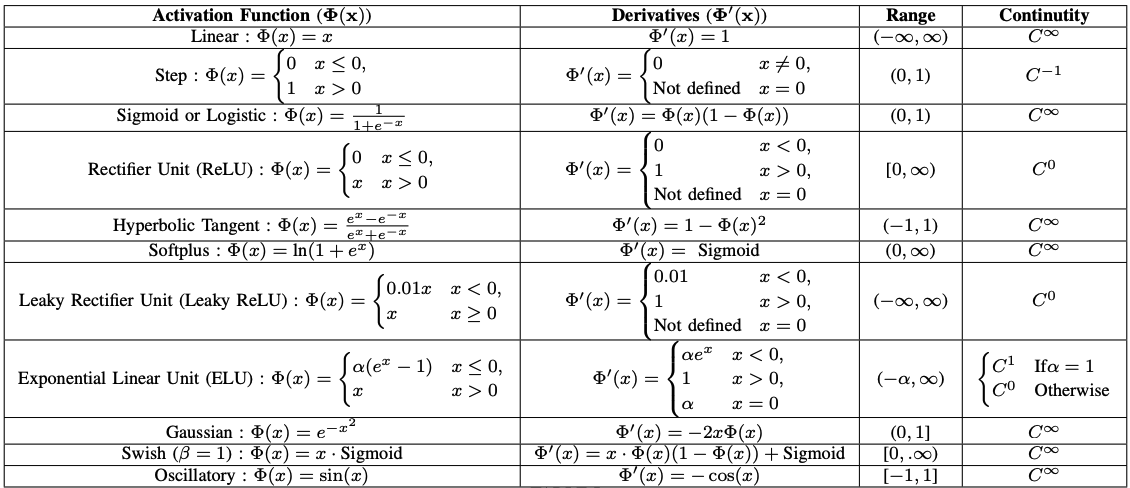
\includegraphics{ActFunTable}
\caption{Common activation functions, their derivatives, range, and order of continuity.}
\end{figure*}
\newpage
\section{Learning}
  \label{sec:Learning}
\subsection{Cost Function}%
  \label{sub:Cost Function}
  Here, we present some common loss functions\cite{ciampiconi2023survey}
\subsection{BackPropagation}%
  \label{sub:BackPropagation}
\newpage
    \bibliographystyle{plainnat}
\bibliography{ML_Report_DRP2024}
  
\end{document} 
